\section{Introduction}

\subsection{Motivation}

Approximately one third of epilepsies are drug-resistant.
If the \ac{EZ}, i.e., ``the area of cortex indispensable for the generation of clinical seizures'' \cite{rosenow_presurgical_2001}, can be localized, resective surgery to remove the \ac{EZ} may be curative.
As previously mentioned, only 40\,\% to 70\,\% of patients with refractory focal epilepsy are seizure-free after surgery \cite{jobst_resective_2015}.
This is, in part, due to limitations identifying the \ac{EZ} during the presurgical evaluation.
Retrospective studies relating presurgical clinical features and resected brain structures to surgical outcome provide useful insights to guide \ac{EZ} resection \cite{jobst_resective_2015}.
To quantify resected structures, first, the resection cavity must be segmented on the postoperative \ac{MRI}.
A preoperative image with a corresponding brain parcellation can then be registered to the postoperative \ac{MRI} to identify resected structures (\cref{fig:resection_diagram}).

\begin{figure}
  \centering
  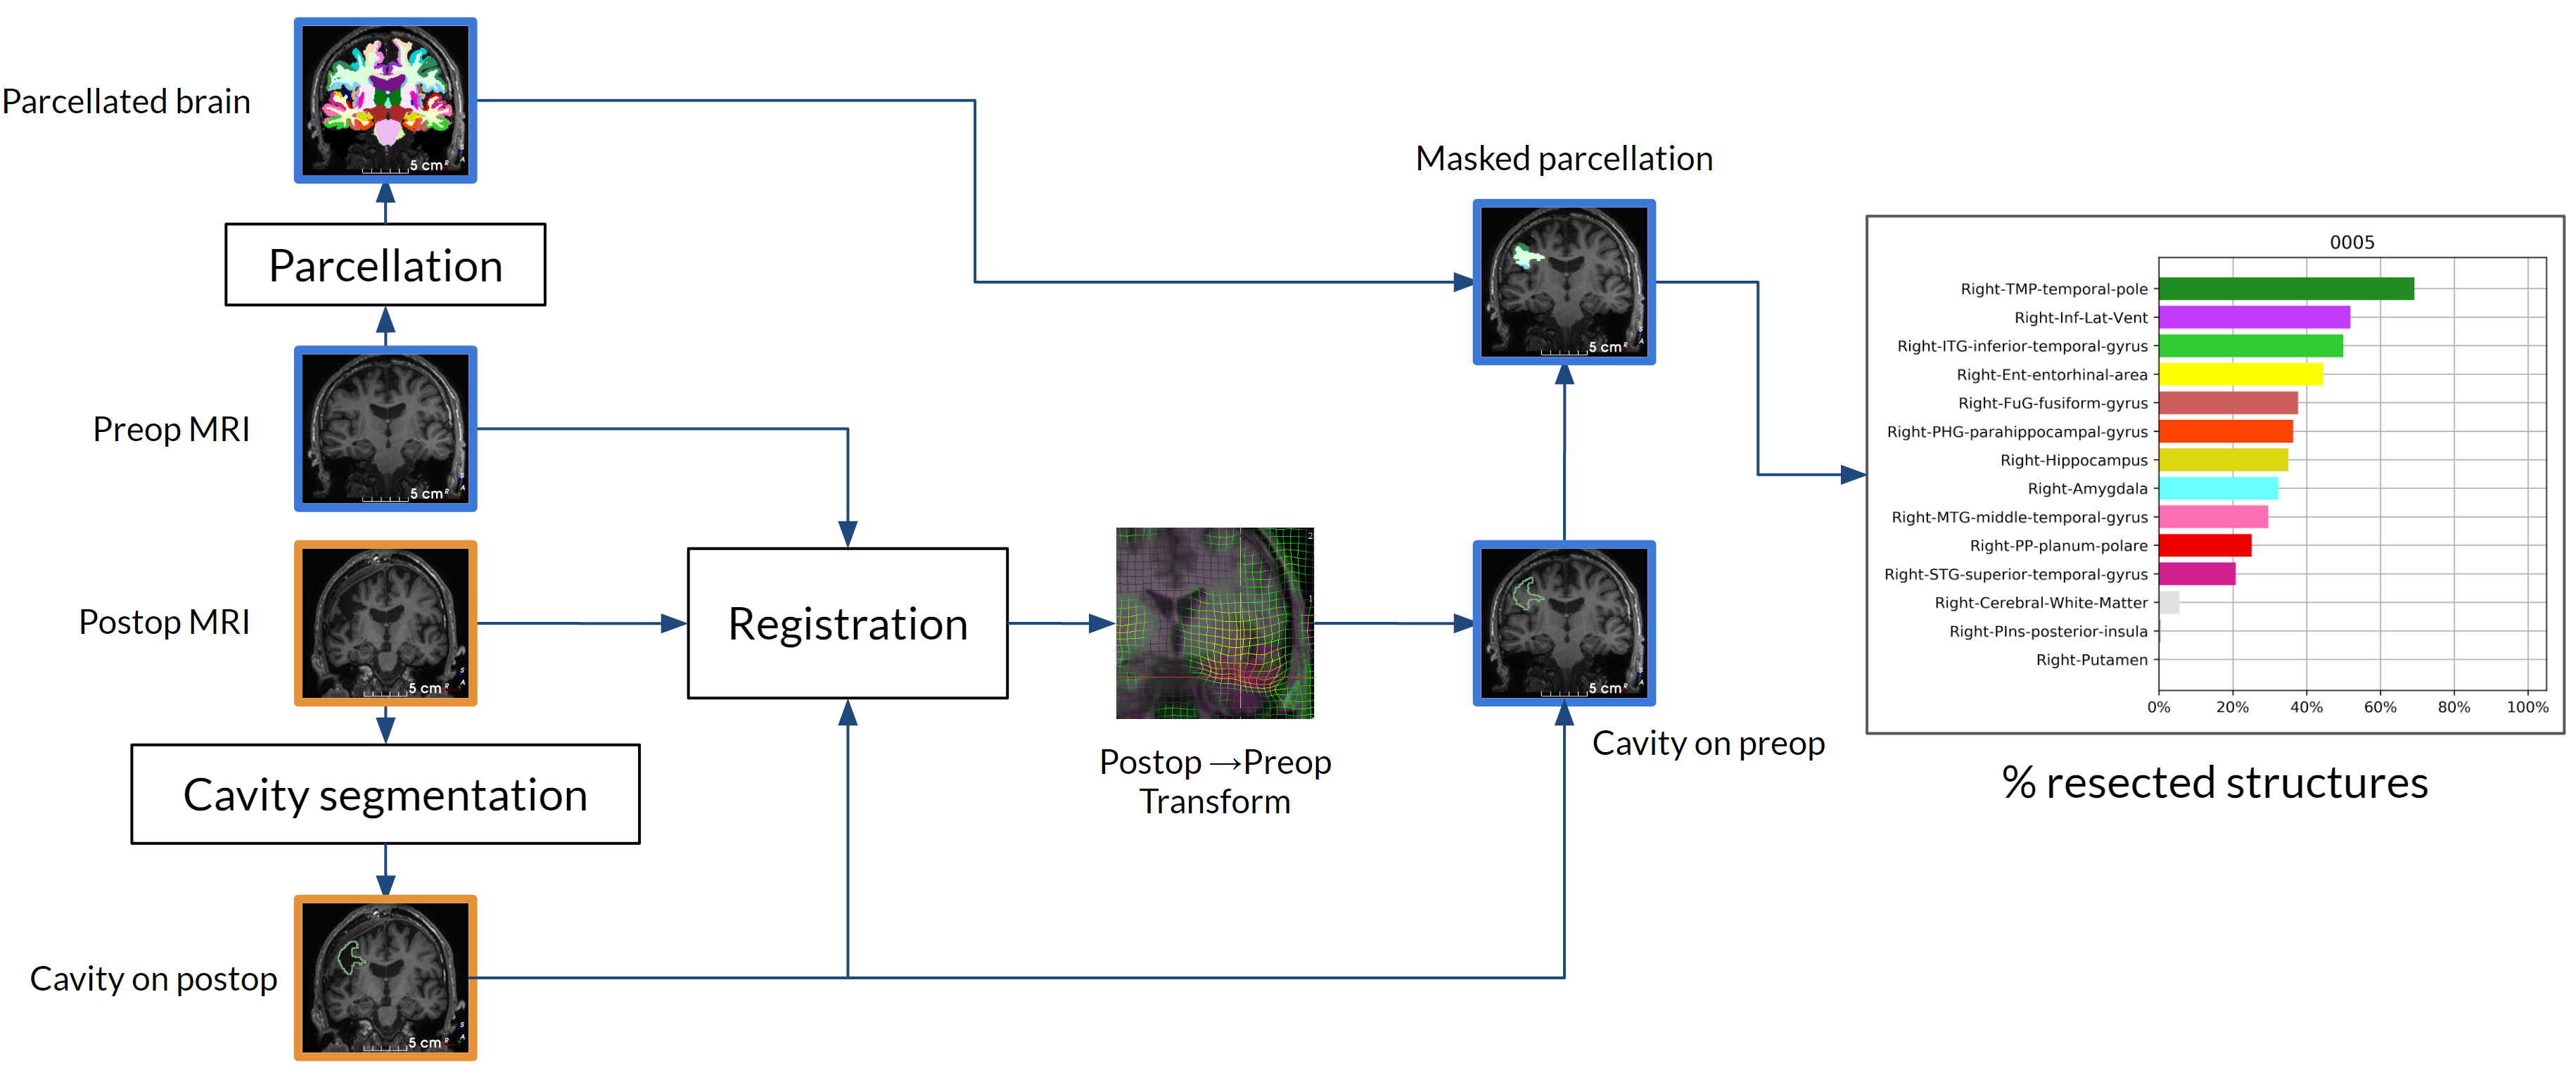
\includegraphics[width=\linewidth]{from_slides/resection_diagram}
  \caption[Diagram of a pipeline to compute resected structures]{
    Diagram of an automatic image processing pipeline used to compute resected structures from a preoperative \ac{MRI} and a postoperative \ac{MRI}.
    In this work, we focus on the elements marked in orange, at the bottom left of the diagram.
  }
  \label{fig:resection_diagram}
\end{figure}

Resection cavity segmentation is also necessary in other applications.
For neuro-oncology, the gross tumor volume, which is the sum of the resection cavity and residual tumor volumes, is estimated for postoperative radiotherapy \cite{ermis_fully_2020}.

Manual segmentation of images is a time-consuming and tedious process, often prone to intra- and inter-rater variability due to fatigue, data overload, or missing manual steps.
Moreover, it can take multiple hours for a human to perform a segmentation of a single three-dimensional medical image \cite{sharma_automated_2010}.

While resection cavity segmentation may appear a simple task, the resection cavity fills with \ac{CSF}, and there are many \ac{MRI} sequences where \ac{CSF} and brain tissue have no distinct appearance.
Moreover, multiple circumstances make automatic segmentation challenging, such as
variation in intensity range in MR images,
missing preoperative data,
white-matter hypointensities around the resection cavity,
small cavities (e.g., with size comparable to a sulcus),
brain shift due to perioperative \ac{CSF} leakage,
postoperative edema,
other tissues present in the cavity (e.g., blood clots),
arachnoid cysts,
brain atrophy,
presence of large ventricles, or
union of lateral ventricle and cavity.
\Cref{fig:hard_resections} shows multiple examples of challenging images.

\begin{figure}
  % \centering

  \begin{subfigure}{0.49\textwidth}
    \centering
    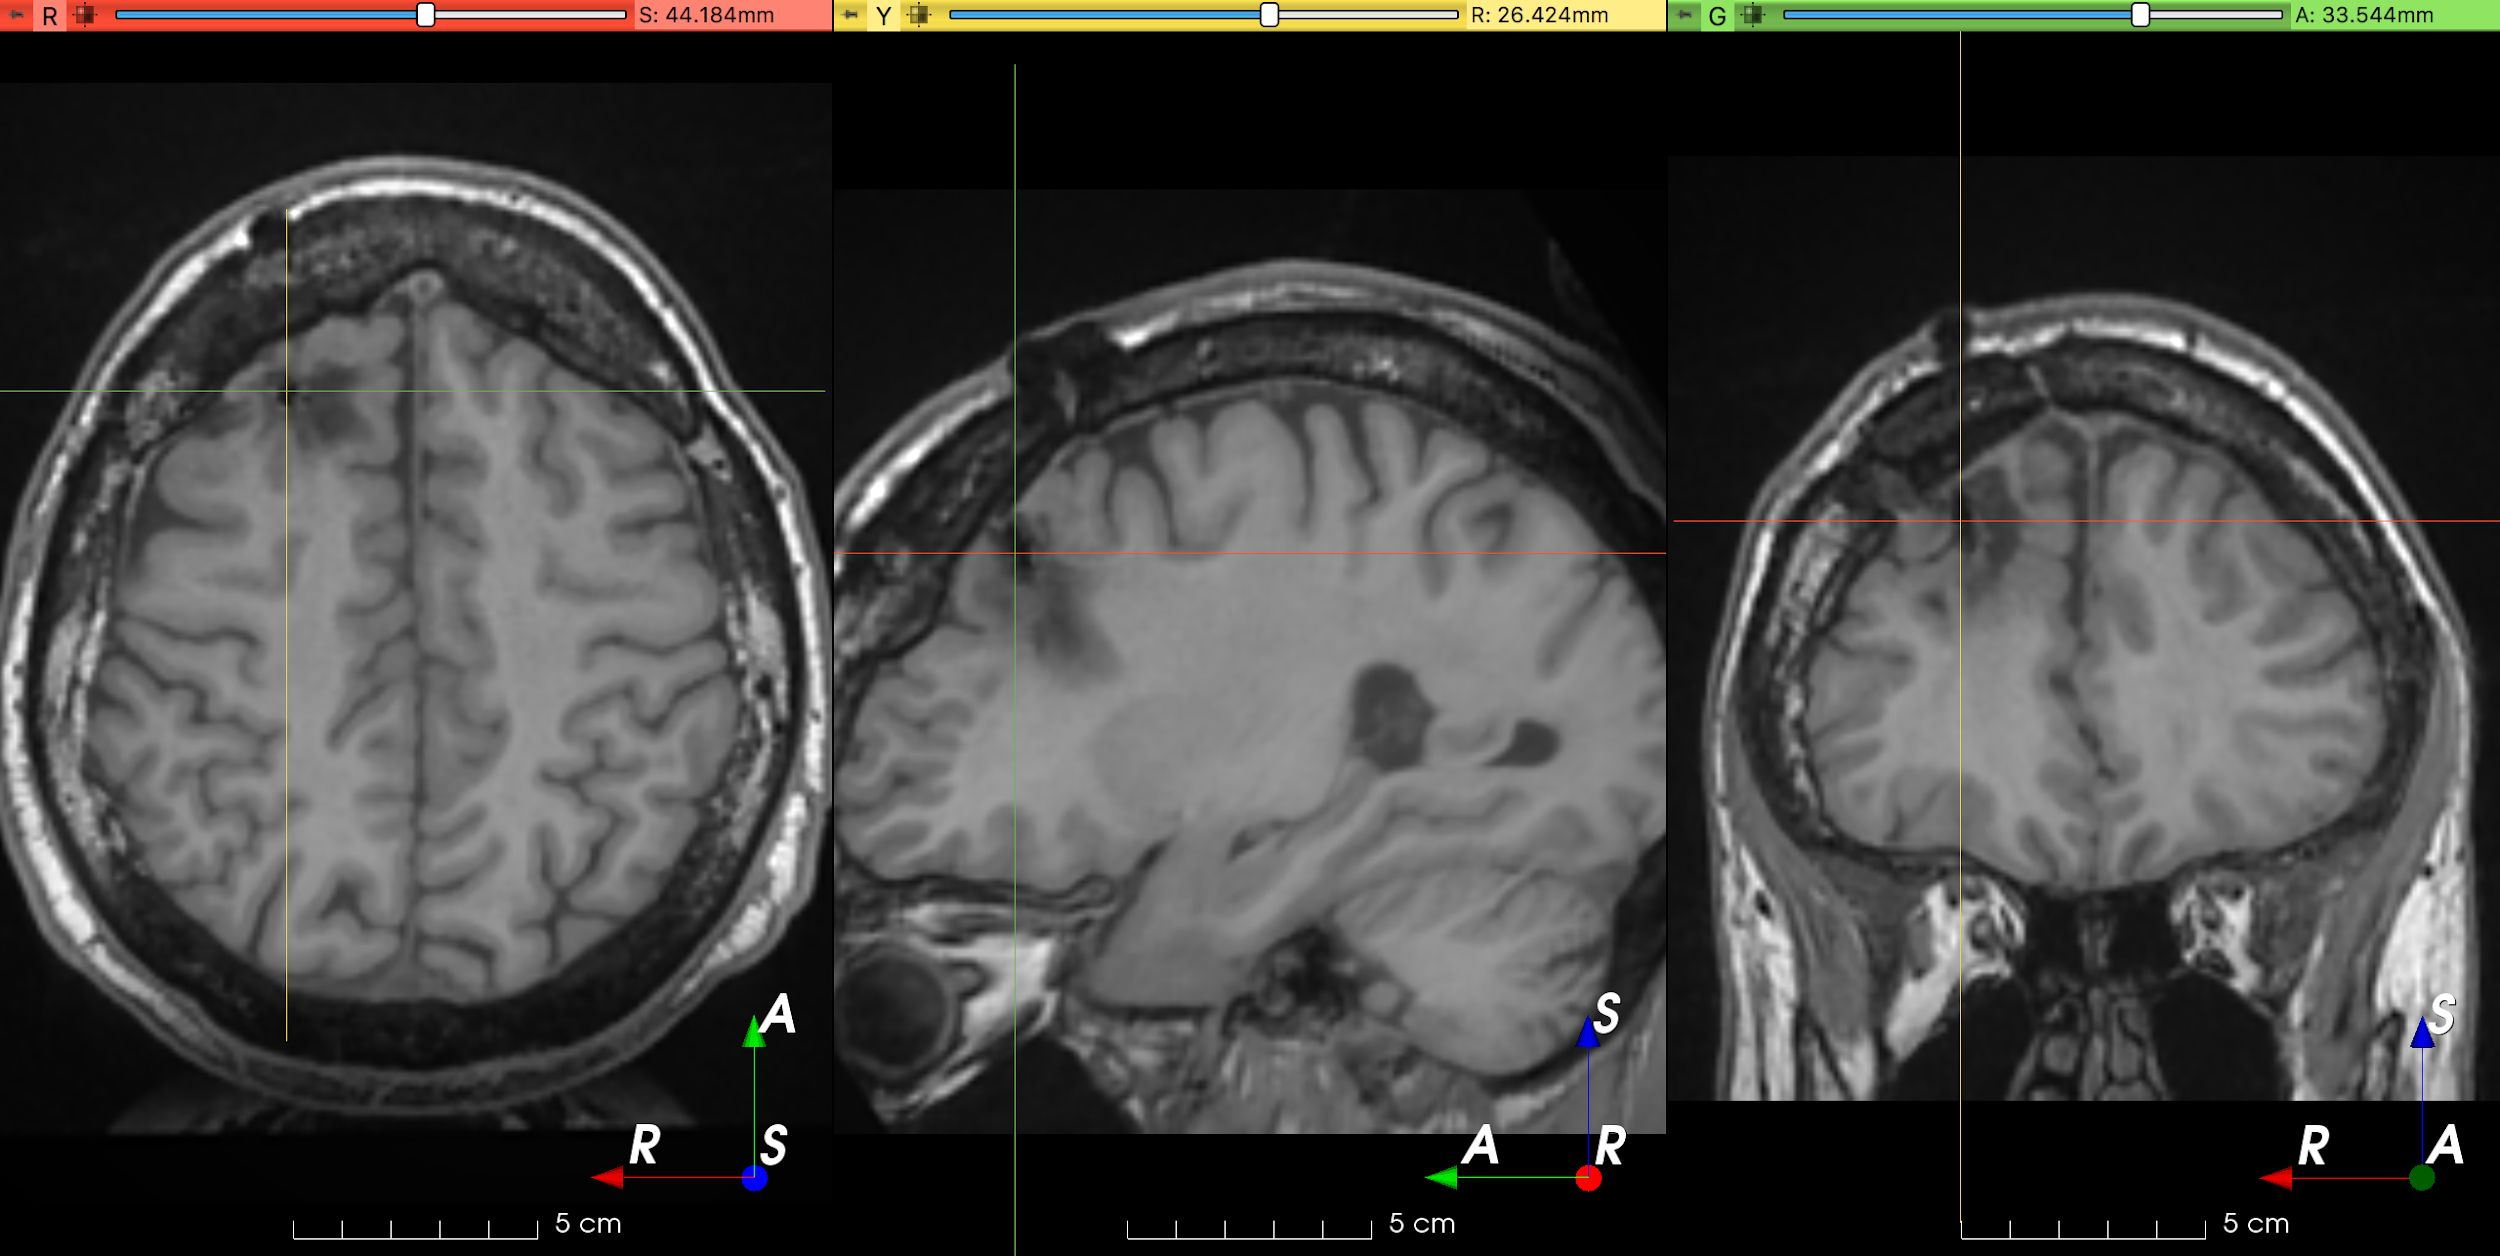
\includegraphics[width=\linewidth]{figures/hard_0}
    \caption{Small frontal lesionectomy surrounded by hypointense white matter}
    \label{fig:hard_sub_0}
  \end{subfigure}
  \hfill
  \begin{subfigure}{0.49\textwidth}
    \centering
    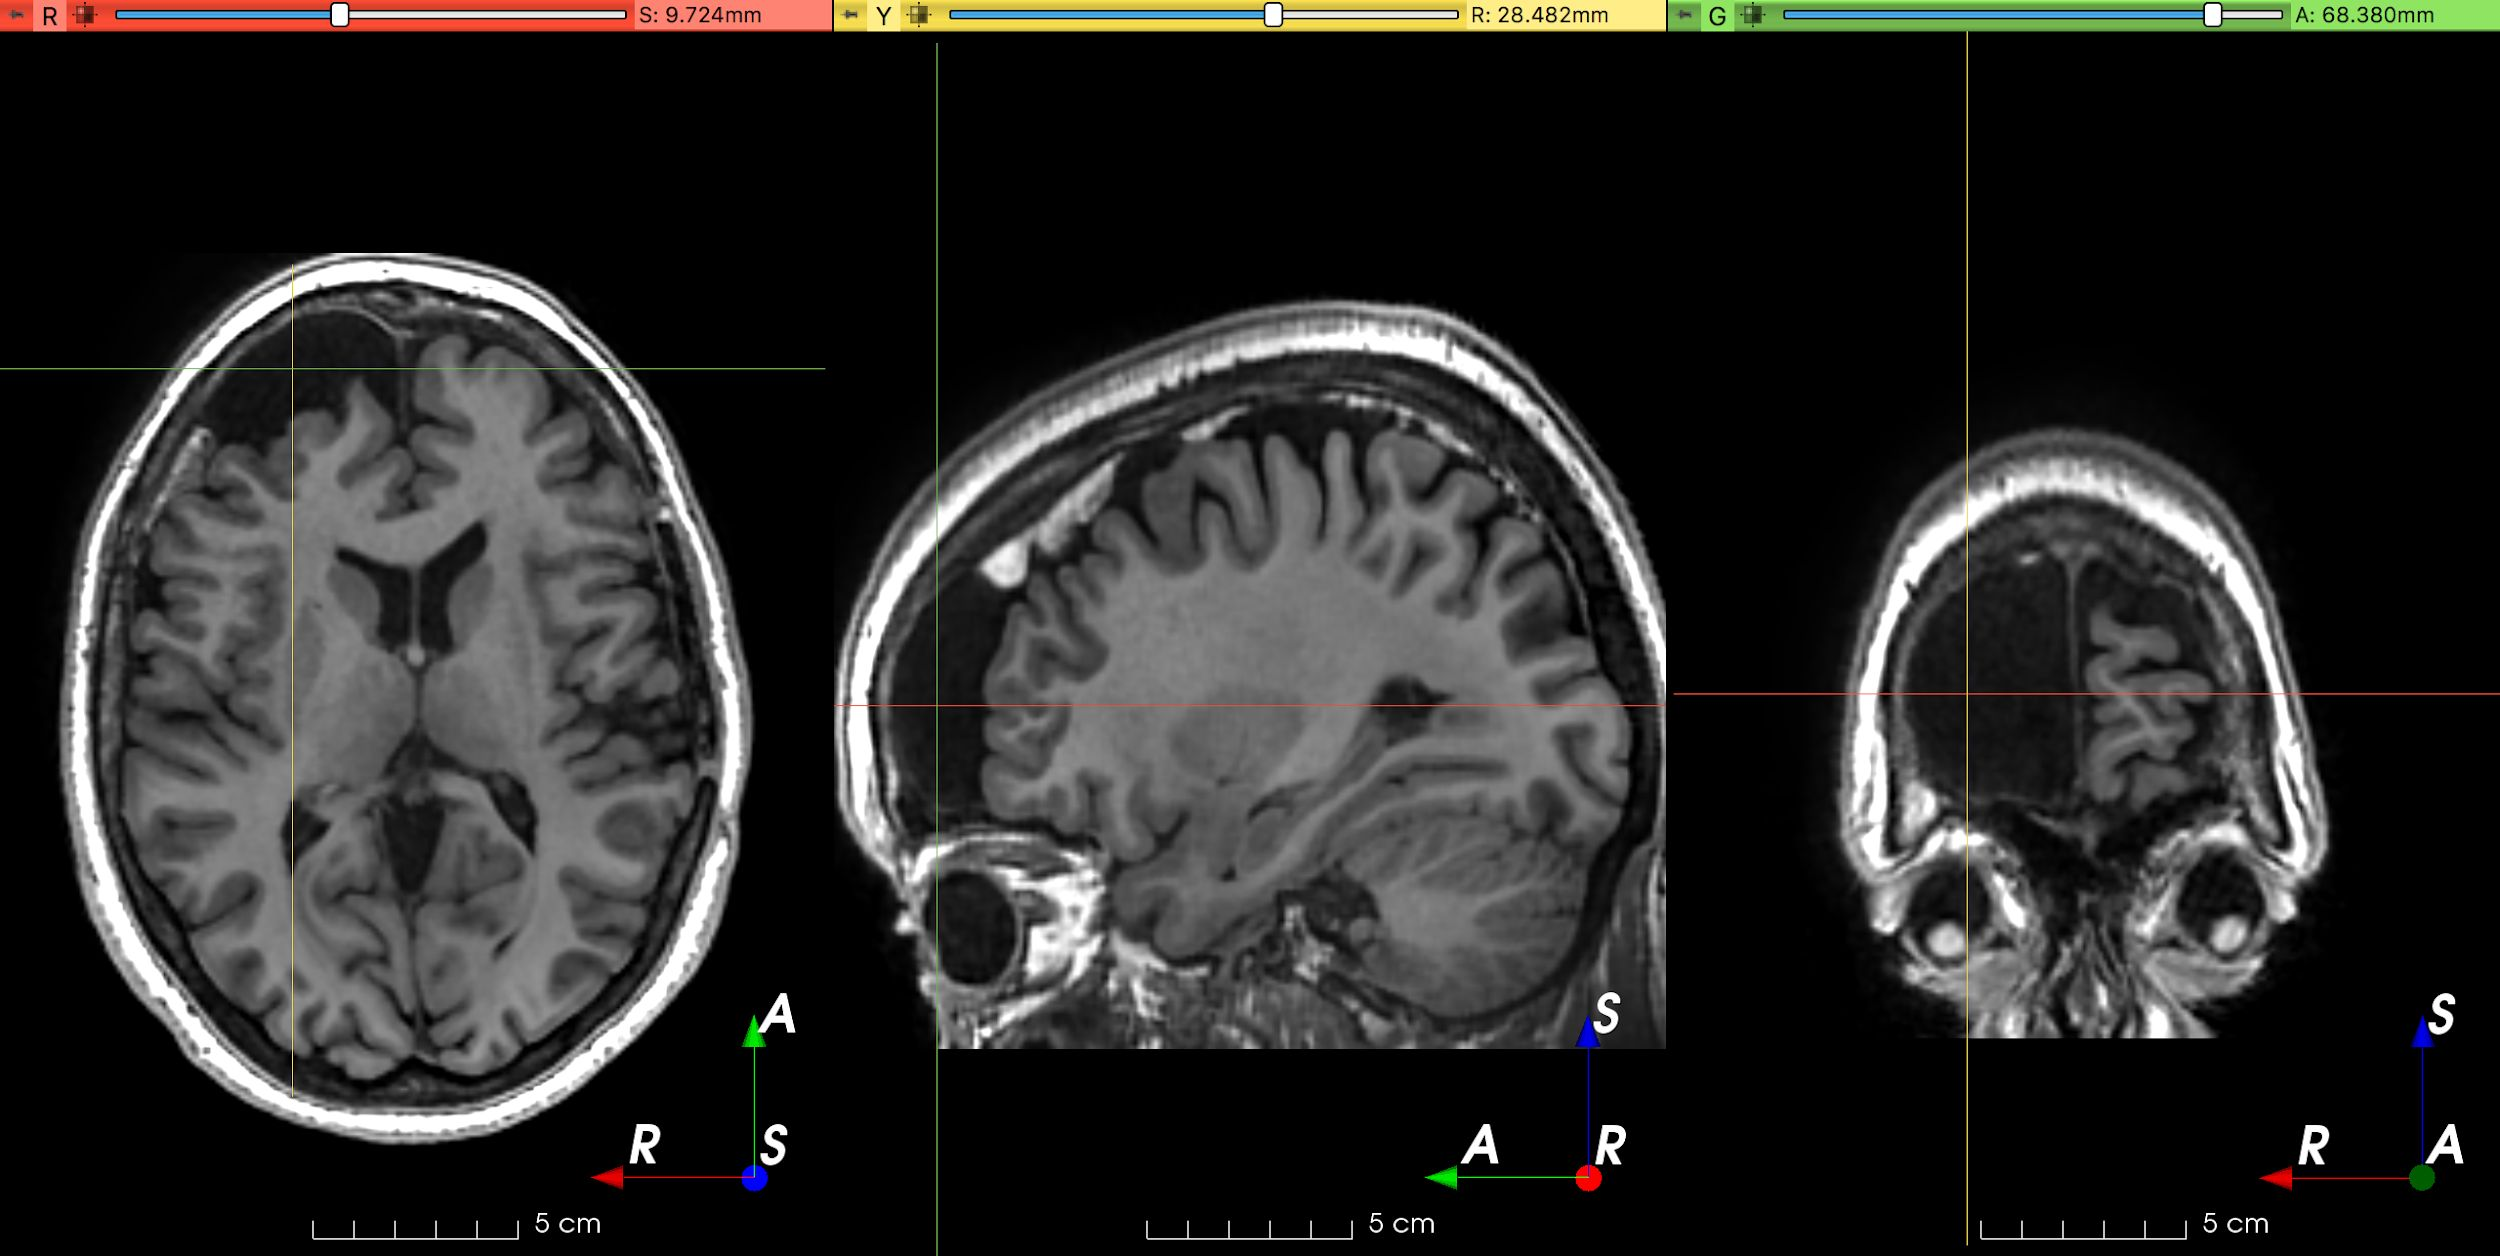
\includegraphics[width=\linewidth]{figures/hard_1}
    \caption{Brain shift after contralateral temporal lobectomy}
    \label{fig:hard_sub_1}
  \end{subfigure}

  \bigskip

  \begin{subfigure}{0.49\textwidth}
    \centering
    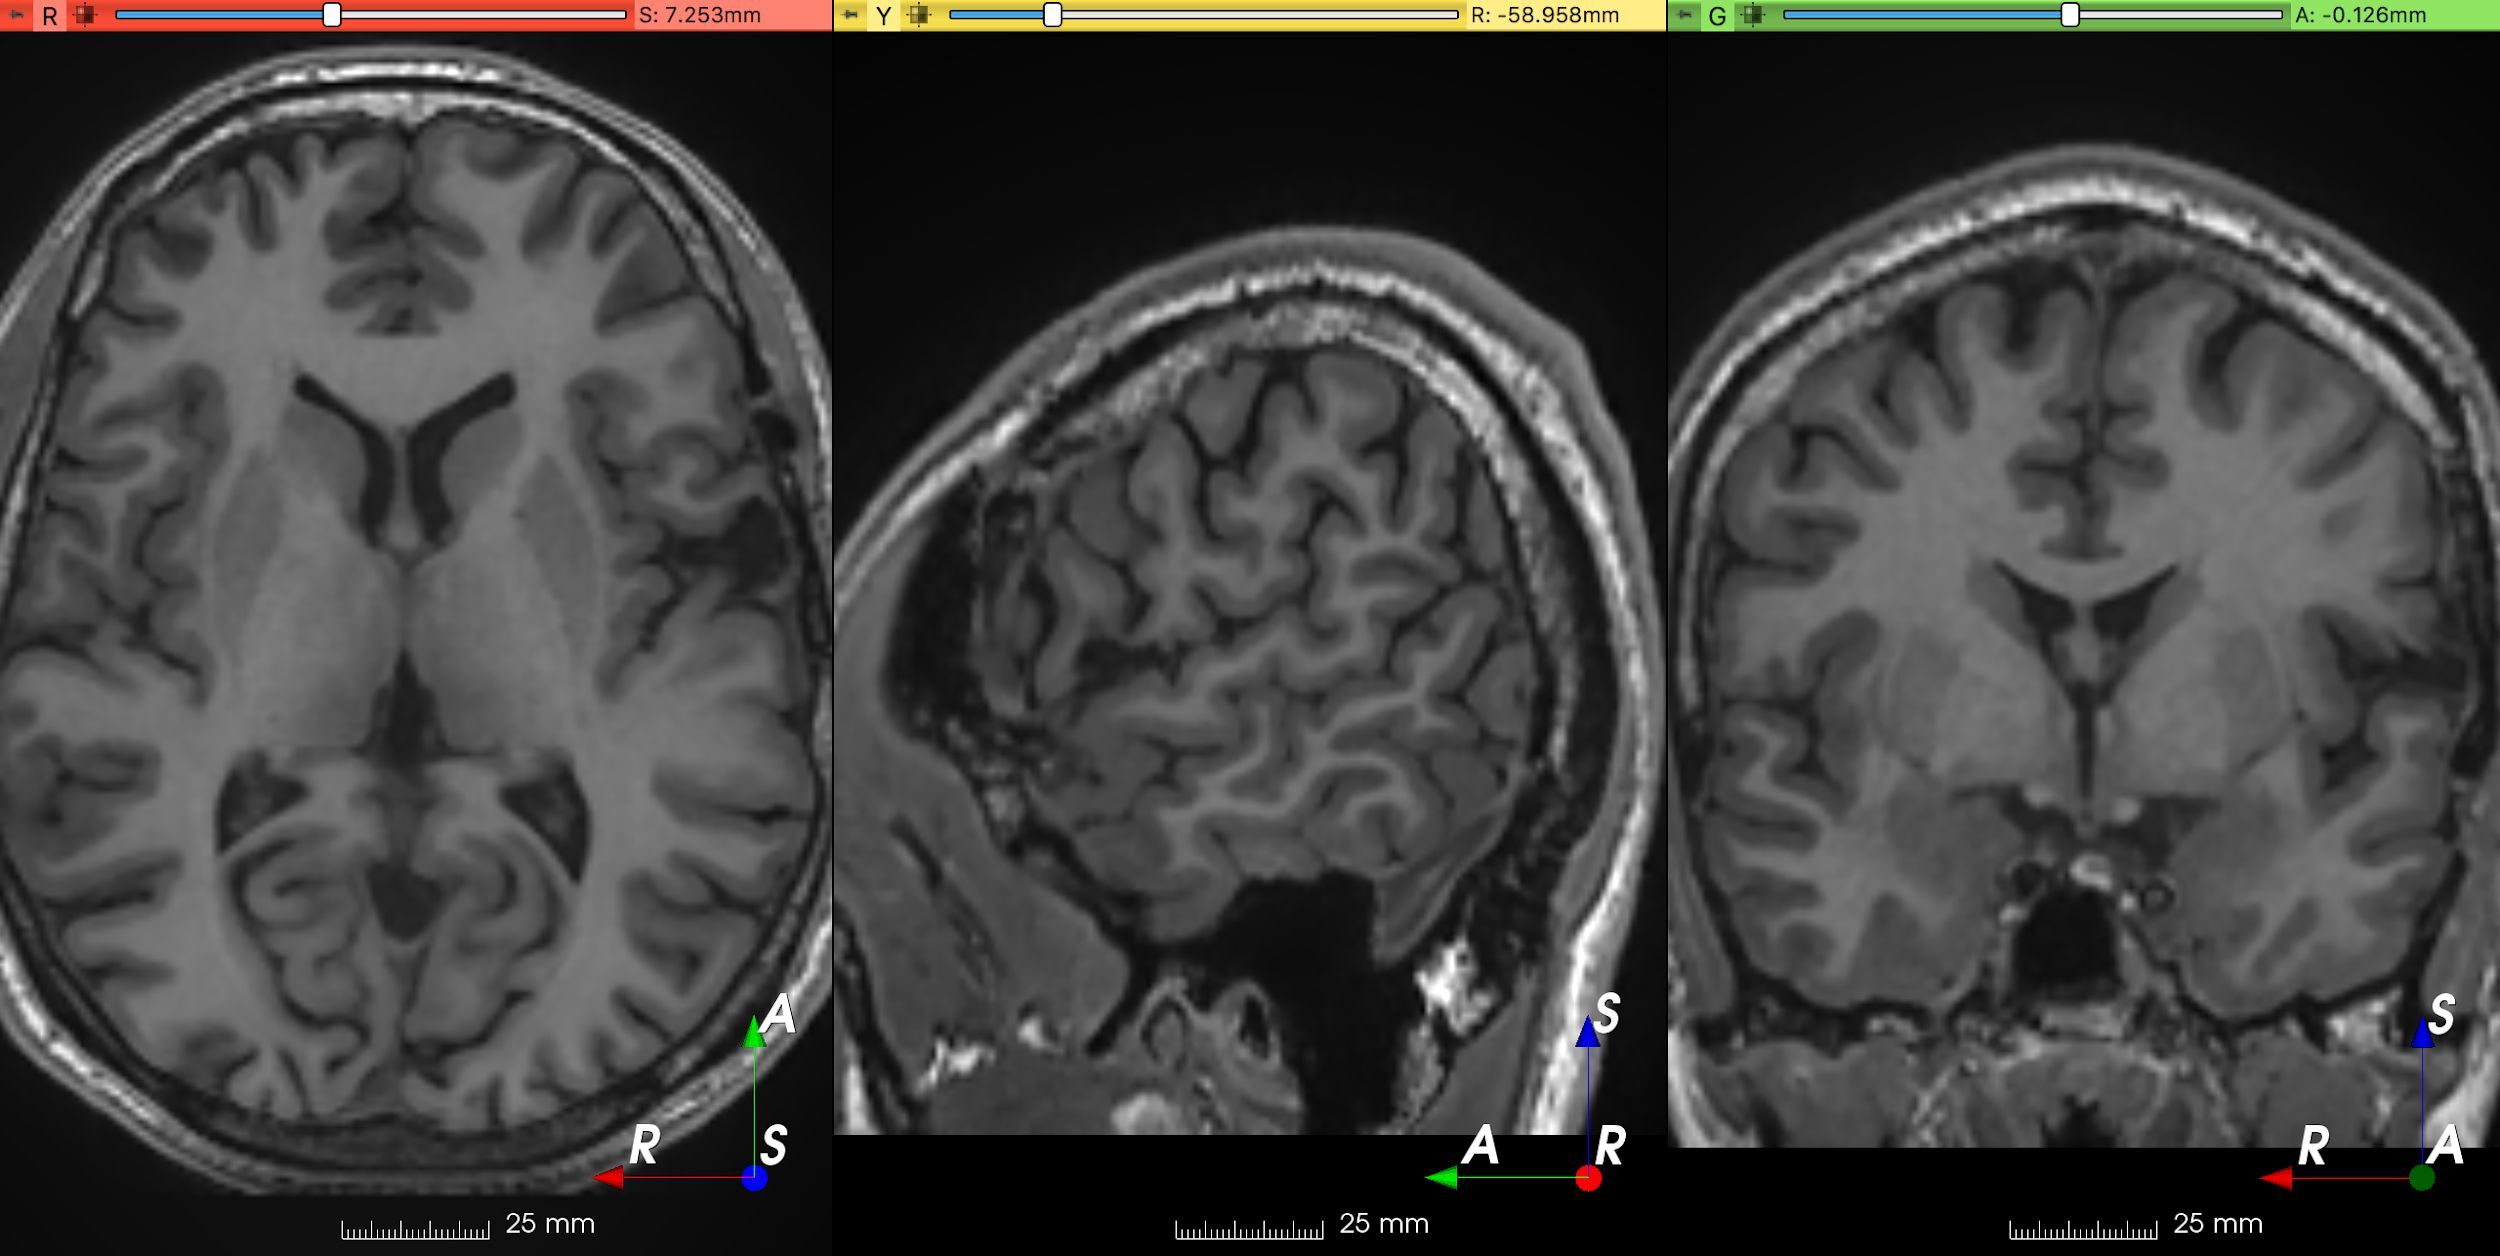
\includegraphics[width=\linewidth]{figures/hard_3}
    \caption{Small frontal lesionectomy near the Sylvian fissure}
    \label{fig:hard_sub_3}
  \end{subfigure}
  \hfill
  \begin{subfigure}{0.49\textwidth}
    \centering
    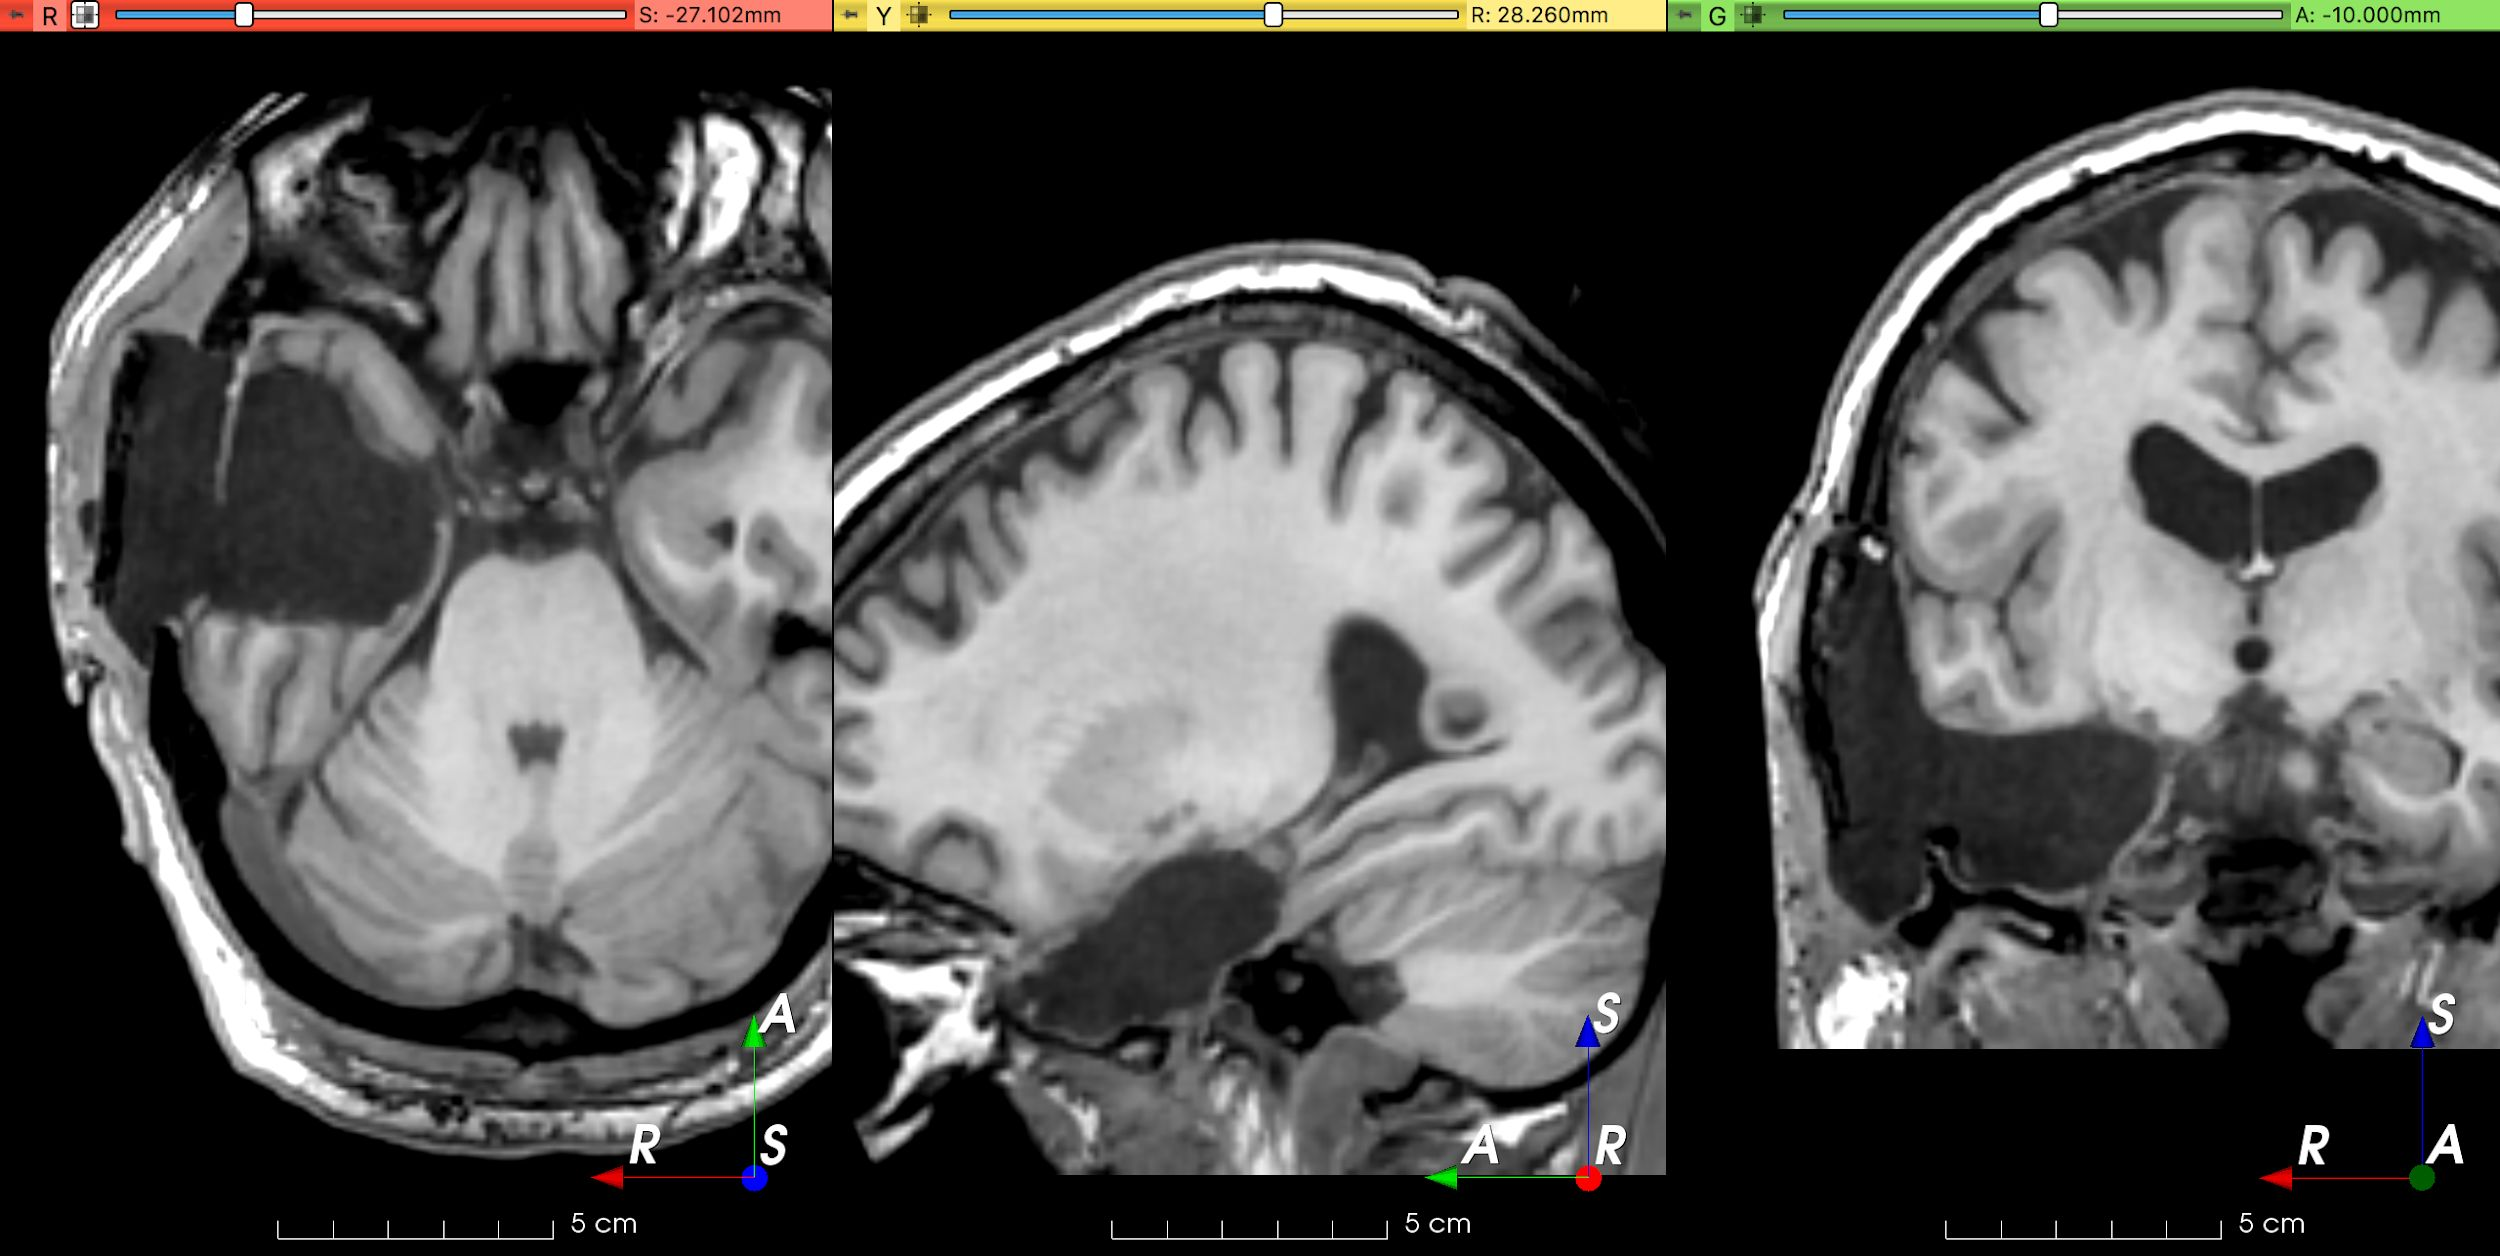
\includegraphics[width=\linewidth]{figures/hard_4}
    \caption{Lack of boundaries between edema and resection cavity}
    \label{fig:hard_sub_4}
  \end{subfigure}

  \bigskip

  \begin{subfigure}{0.49\textwidth}
    \centering
    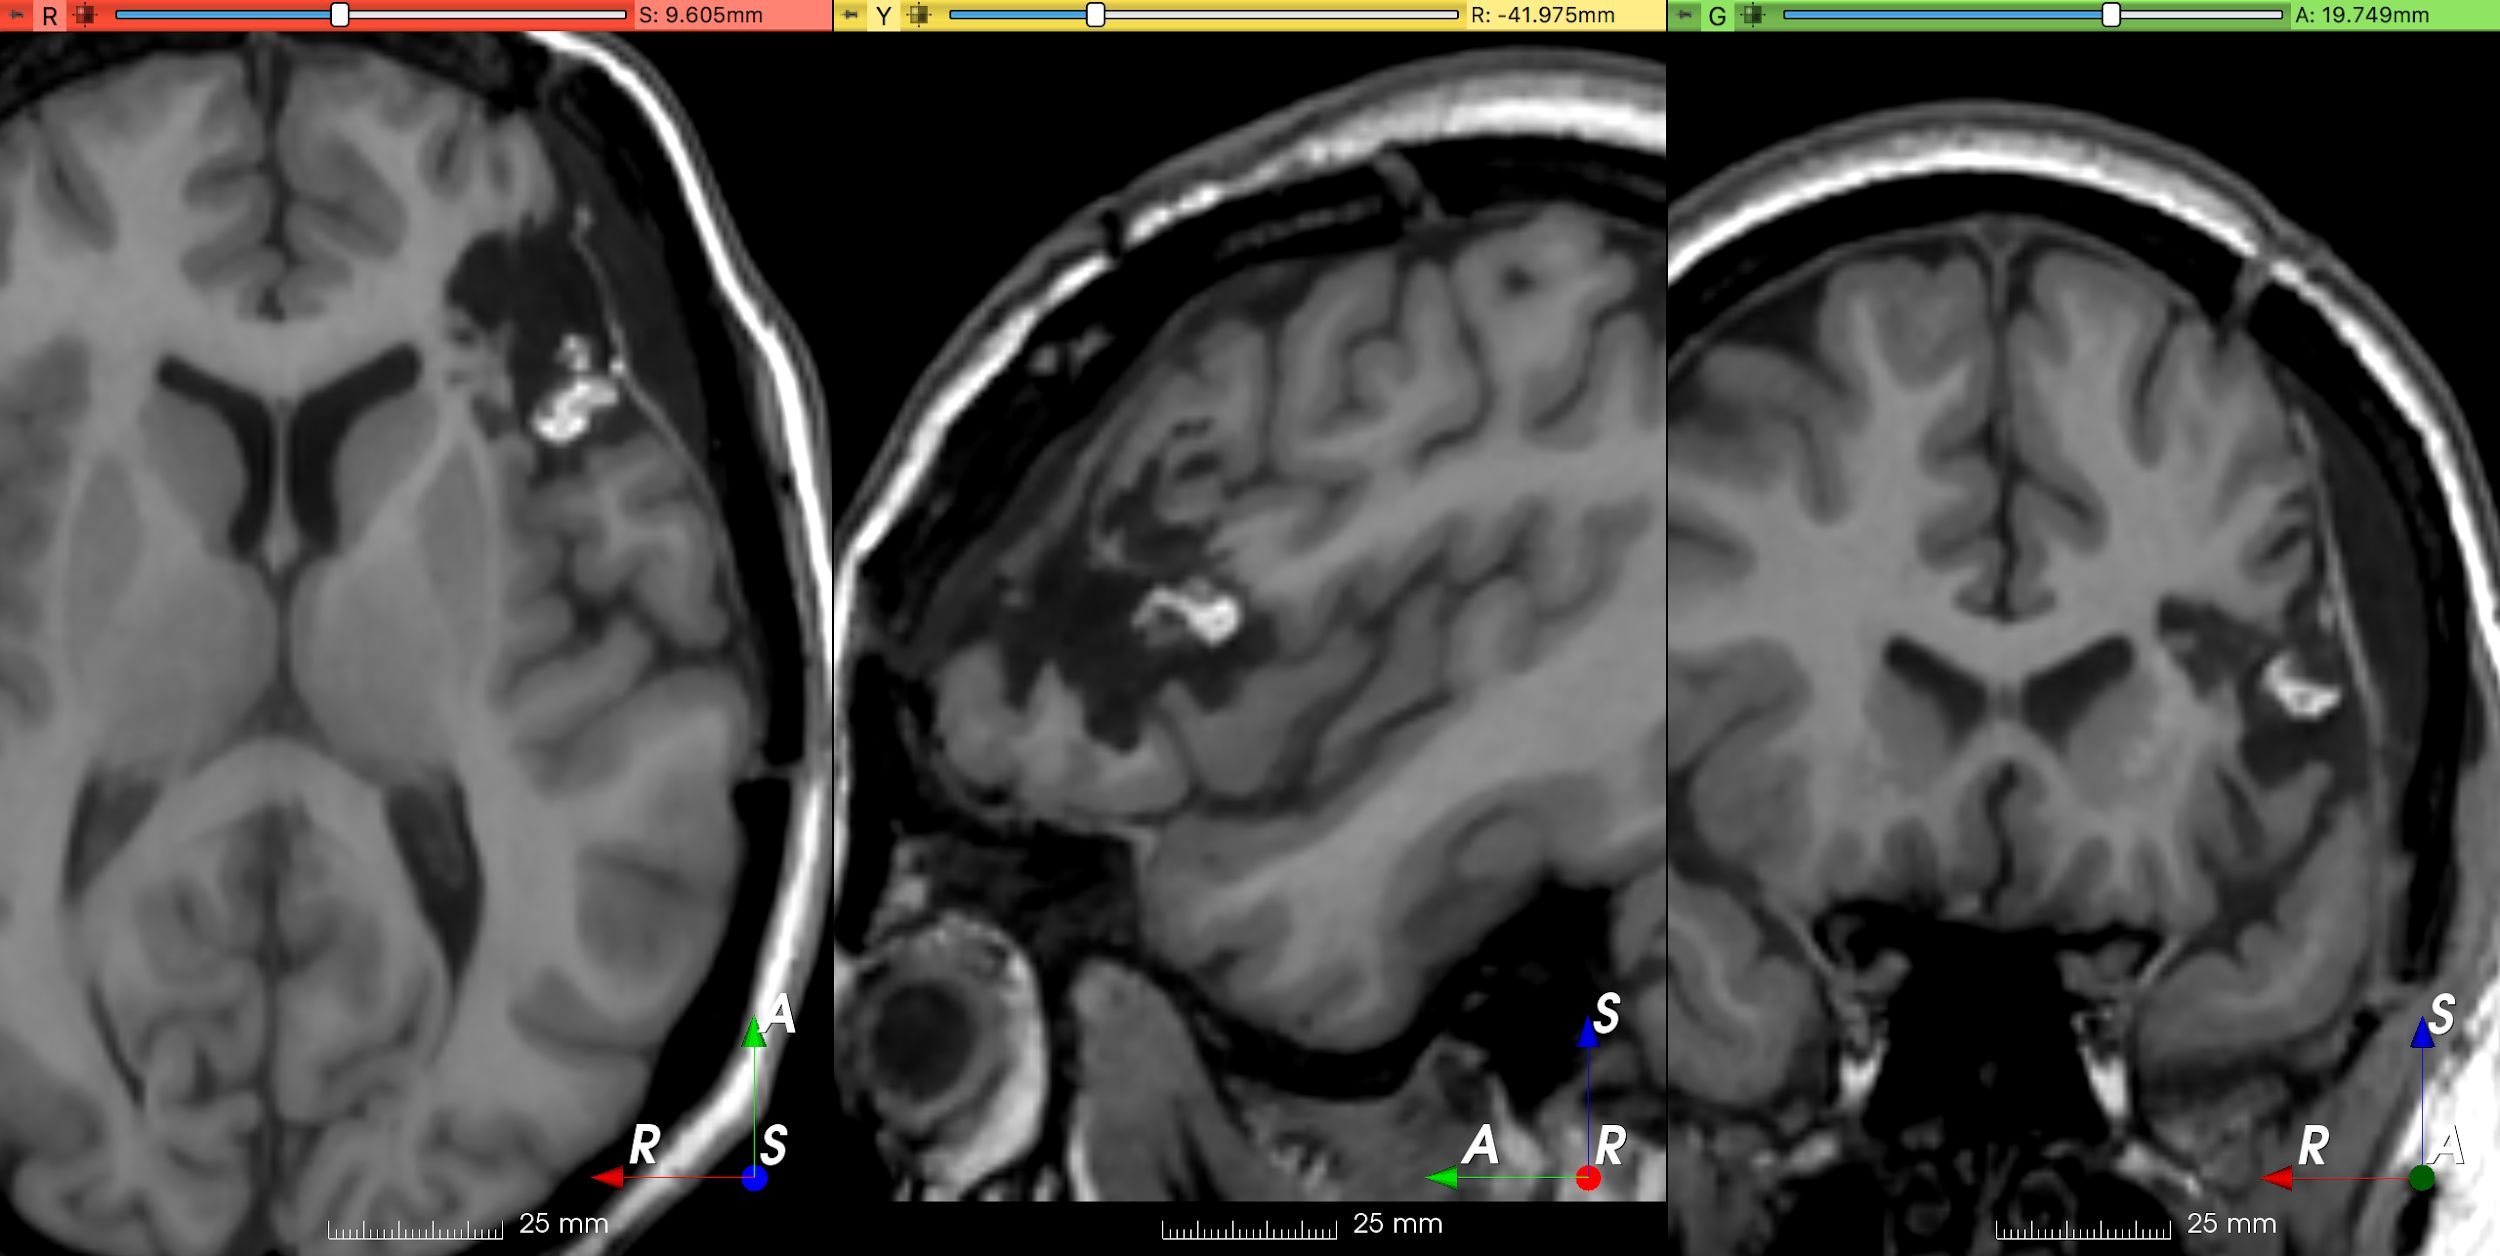
\includegraphics[width=\linewidth]{figures/hard_5}
    \caption{Possible blood clot within the cavity}
    \label{fig:hard_sub_5}
  \end{subfigure}
  \hfill
  \begin{subfigure}{0.49\textwidth}
    \centering
    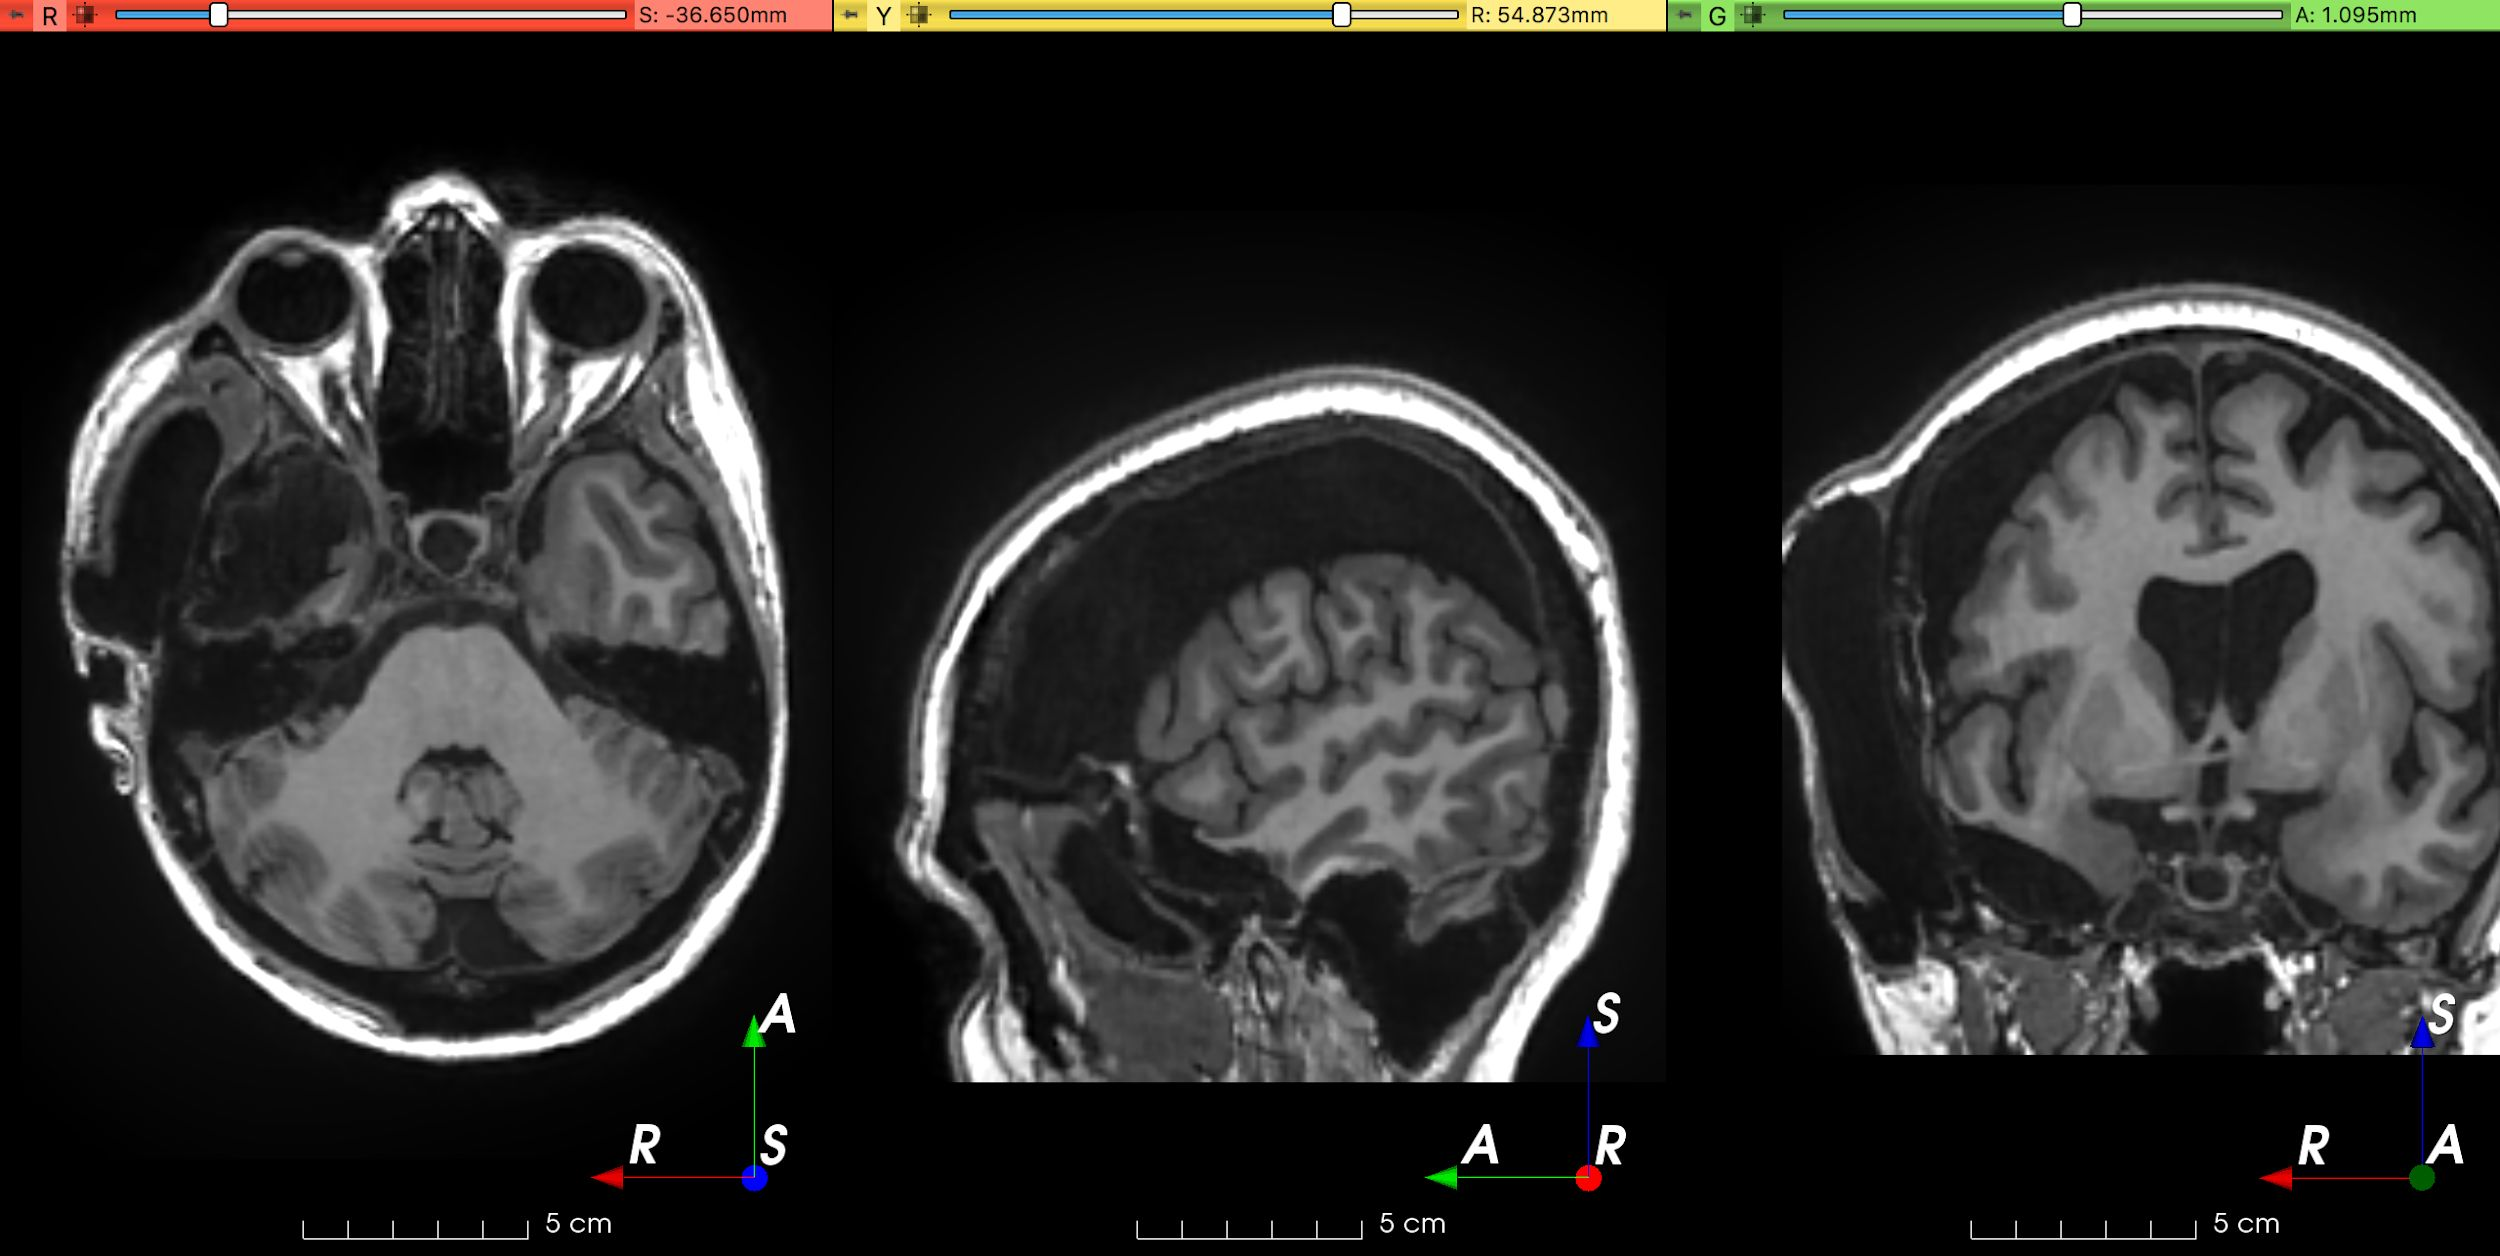
\includegraphics[width=\linewidth]{figures/hard_6}
    \caption{Brain shift, edema and resection cavity}
    \label{fig:hard_sub_6}
  \end{subfigure}

  \bigskip

  \begin{subfigure}{0.49\textwidth}
    \centering
    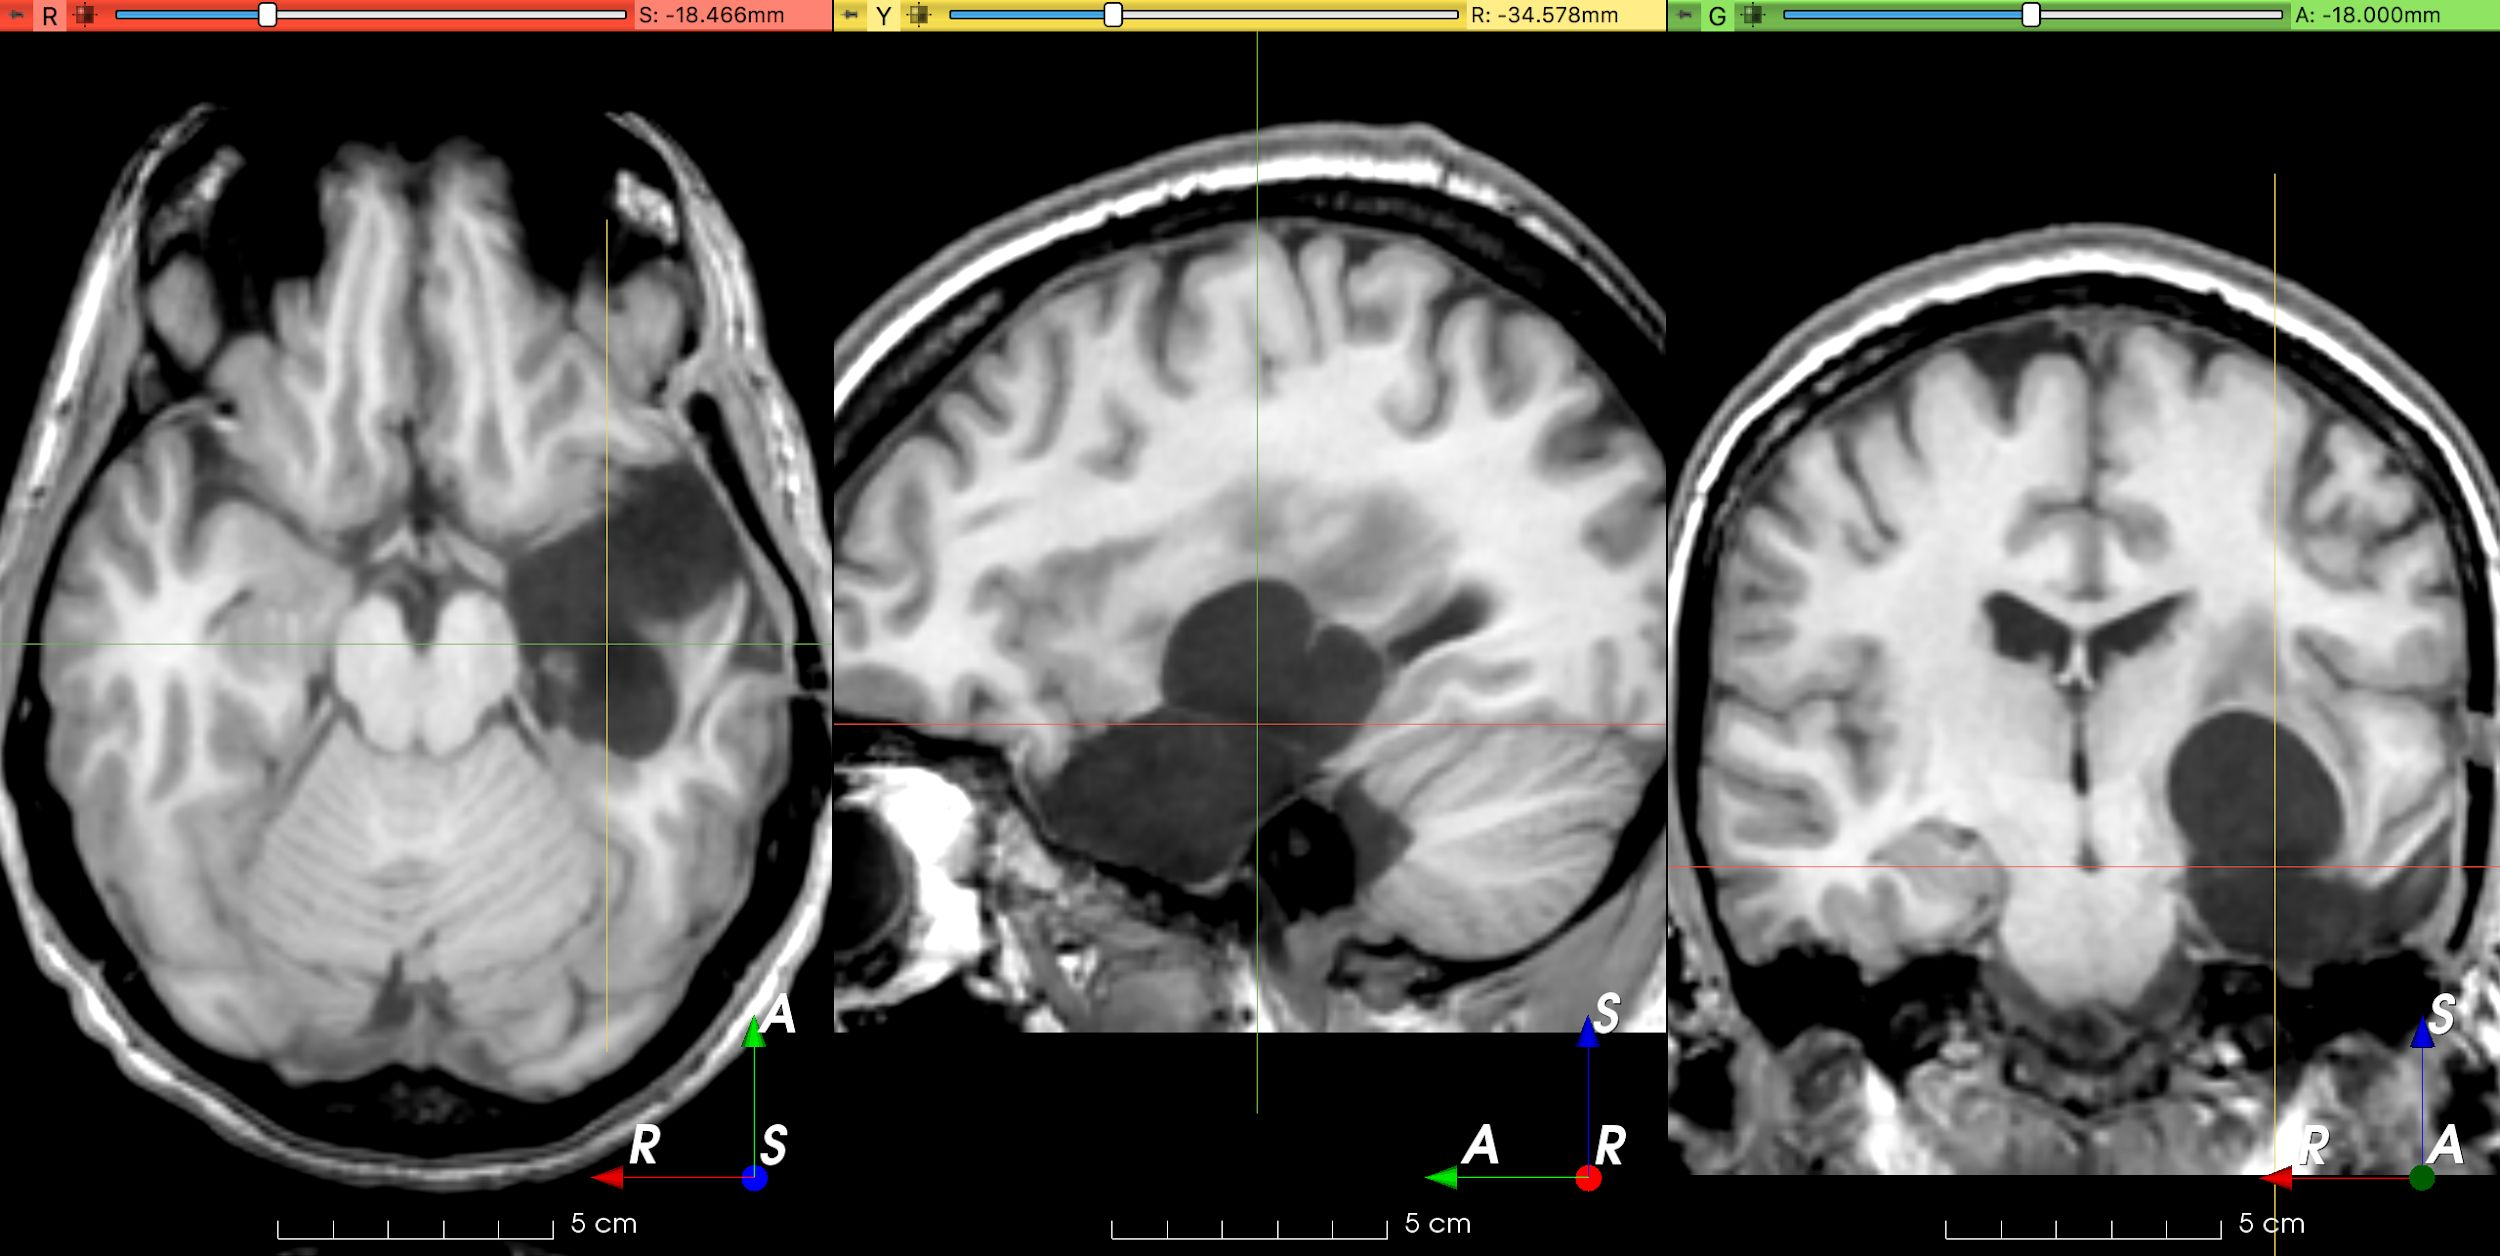
\includegraphics[width=\linewidth]{figures/hard_7}
    \caption{Arachnoid cyst and resection cavity}
    \label{fig:hard_sub_7}
  \end{subfigure}
  \hfill
  \begin{subfigure}{0.49\textwidth}
    \centering
    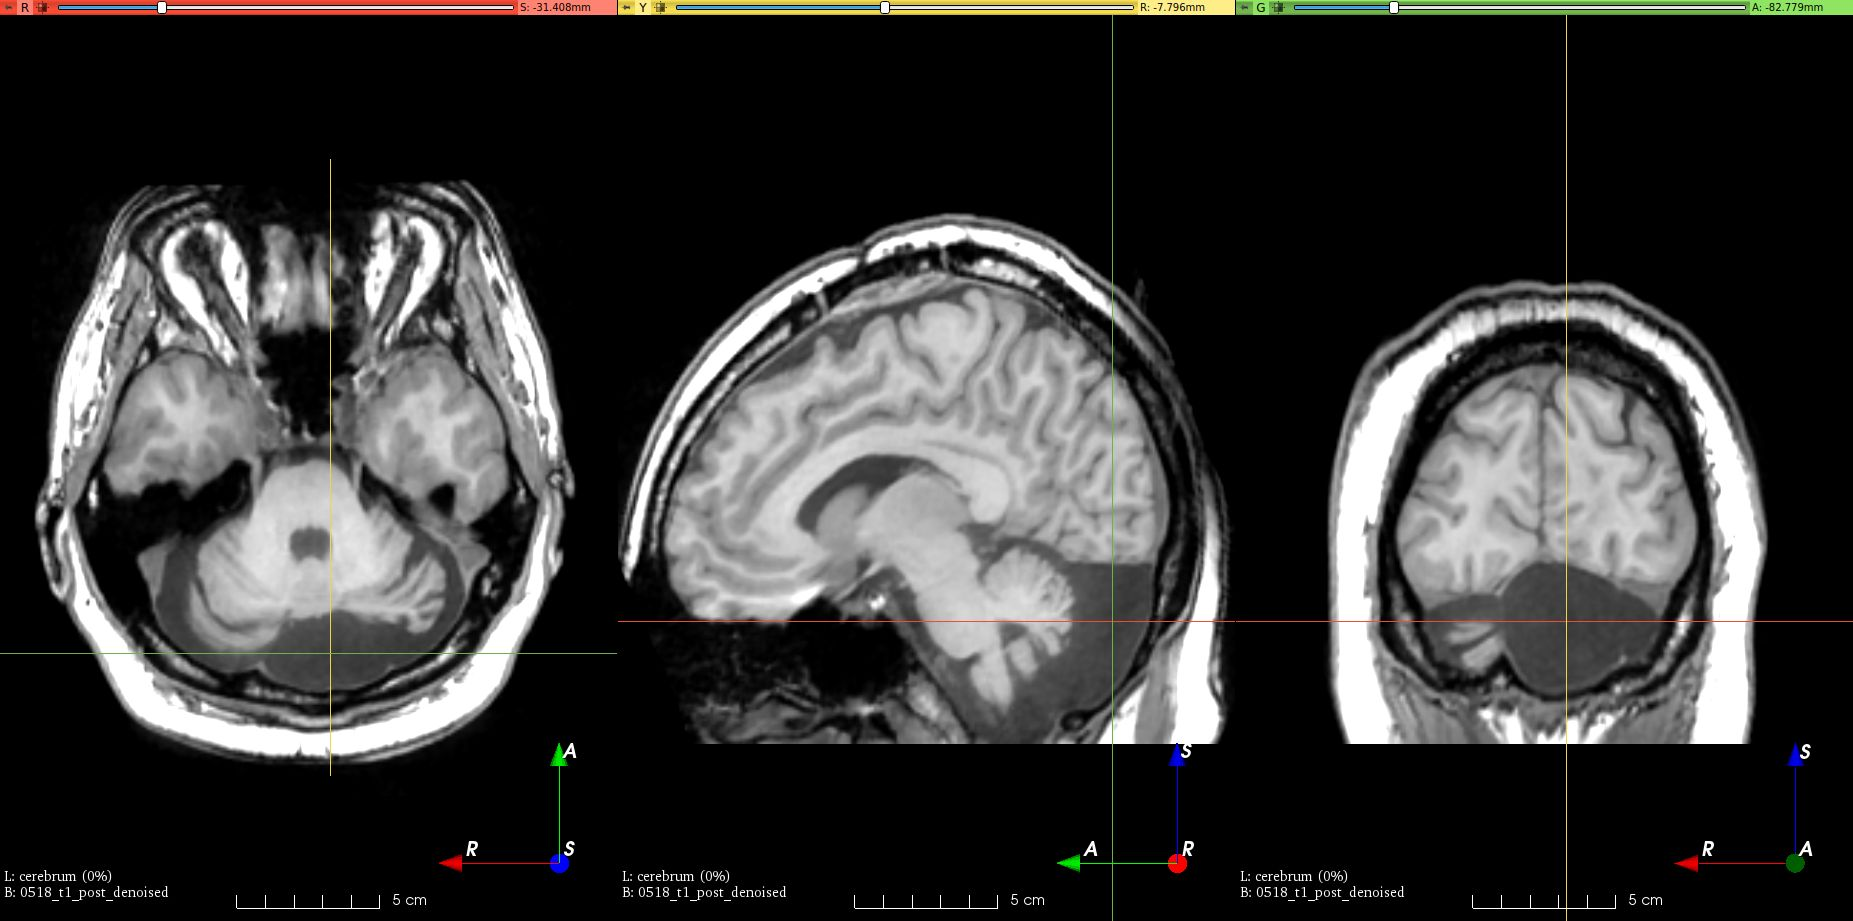
\includegraphics[width=\linewidth]{figures/hard_8}
    \caption{Cerebellar degeneration}
    \label{fig:hard_sub_8}
  \end{subfigure}

  \caption{
    Examples of challenging cases for segmentation of resection cavities.
  }
  \label{fig:hard_resections}
\end{figure}

Despite recent efforts to segment resection cavities in the context of brain cancer \cite{meier_automatic_2017,ermis_fully_2020}, little research has been published in the context of epilepsy surgery.
Furthermore, previous work is limited by the lack of benchmark datasets, released code or trained models, and evaluation is restricted to single-institution datasets used for both training and testing.


\subsection{Related works}

After surgery, resection cavities fill with \ac{CSF}.
This causes an inherent uncertainty in delineating resection cavities adjacent to structures such as sulci, ventricles or edemas.
Nonlinear registration has been presented to segment the resection cavity for epilepsy \cite{chitphakdithai_non-rigid_2010} and brain tumor \cite{chen_deformable_2015} surgeries by detecting non-corresponding regions between pre- and postoperative images.
However, evaluation of these methods was restricted to a very small number of images.
Furthermore, in cases with intensity changes due to the resection (e.g., brain shift, atrophy, fluid filling), non-corresponding voxels may not correspond to the resection cavity (\cref{fig:missing_correspondences}).

\begin{figure}
  \centering
  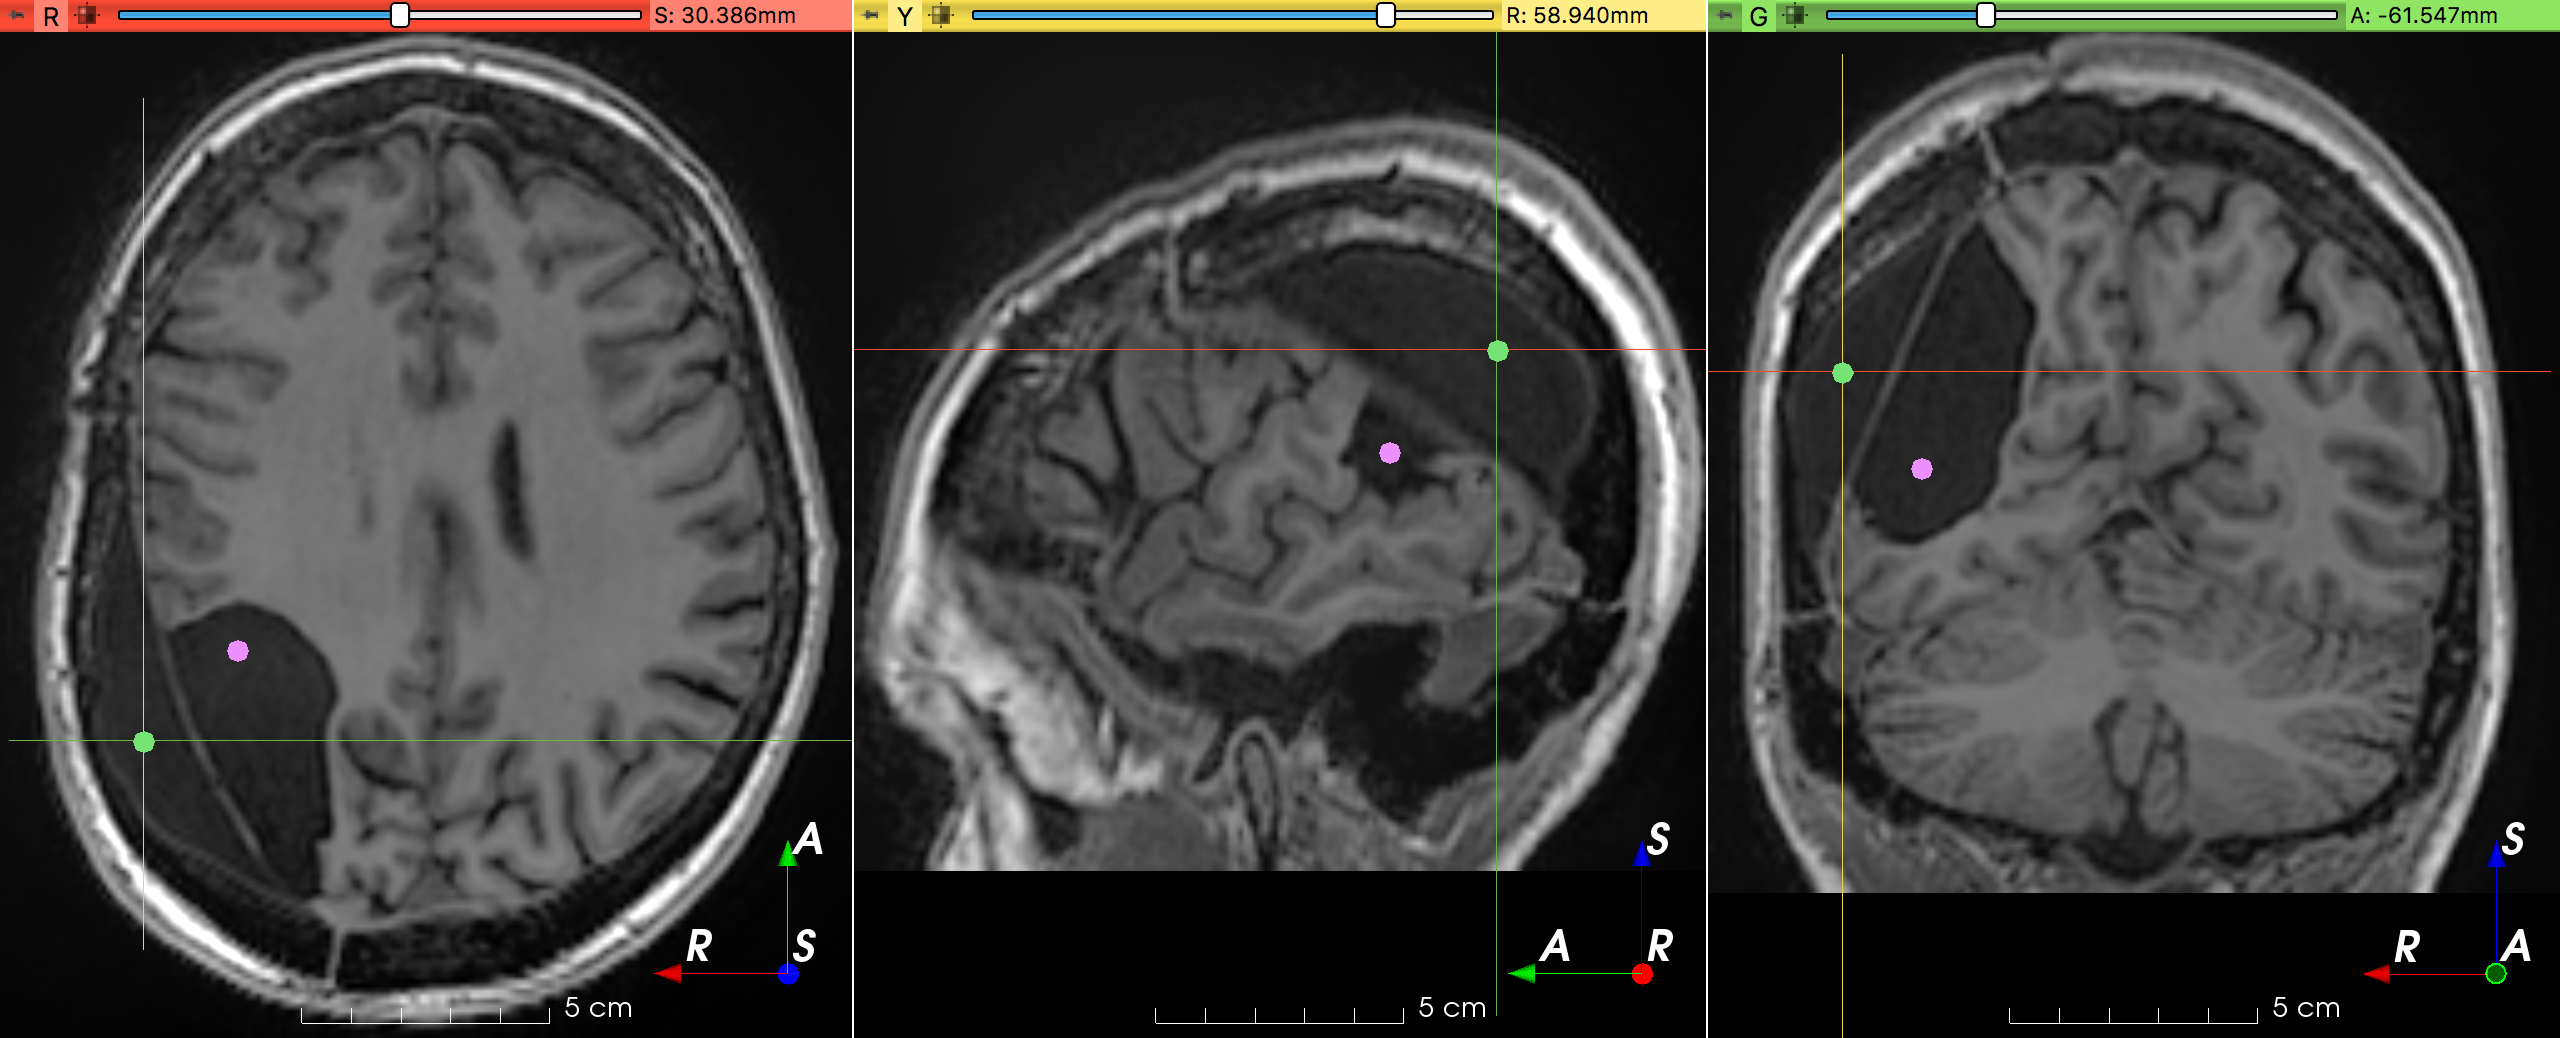
\includegraphics[width=\linewidth]{figures/edema_0985}
  \caption[Example of a patient with postoperative edema]{Example of a patient with postoperative edema (green circle) and resection cavity (pink circle), where registration would be challenging due to missing correspondences between the pre- and post-operative images.}
  \label{fig:missing_correspondences}
\end{figure}

Decision forests were presented for brain cavity segmentation after glioblastoma surgery, using four \ac{MRI} modalities \cite{meier_automatic_2017}.
These methods, which aggregate hand-crafted features extracted from all  modalities to train a classifier, can be sensitive to signal inhomogeneity and unable to distinguish regions with intensity patterns similar to \ac{CSF} from resection cavities.
Recently, a 2D \ac{CNN} was trained to segment the resection cavity on \ac{MRI} slices in 30 glioblastoma patients \cite{ermis_fully_2020}.
They obtained a `median (interquartile range)' \ac{DSC} of 84 (10) compared to ground-truth labels by averaging predictions across anatomical axes to compute the 3D segmentation.
While these approaches require four modalities to segment the resection cavity, some of the modalities are often unavailable in clinical settings \cite{dorent_learning_2021}.
Furthermore, code and datasets are not publicly available, hindering a fair comparison across methods.
Applying these techniques requires curating a dataset with manually obtained annotations to train the models, which is expensive.

Unsupervised learning methods can leverage large, unlabeled medical image datasets during training.
In self-supervised learning, training instances are generated automatically from unlabeled data and used to train a model to perform a pretext task. %such as inpainting or image restoration.
The model can be fine-tuned on a smaller labeled dataset to perform a downstream task \cite{chen_self-supervised_2019}.
The pretext and downstream tasks may be the same.
For example, a \ac{CNN} was trained to reconstruct a skull bone flap by simulating craniectomies on CT scans \cite{matzkin_self-supervised_2020}.
Lesions simulated in chest CT of healthy subjects were used to train models for nodule detection, improving accuracy compared to training on a smaller dataset of real lesions \cite{pezeshk_seamless_2017}.

% Recovered from long version
Semi-supervised learning may be used when a large amount of unlabeled data is available.
A model trained on a labeled dataset (which may have been generated in a self-supervised setting) can generate pseudolabels for unlabeled data.
Uncertainty estimation may be used to select pseudolabeled instances with a low uncertainty for medical image segmentation tasks, improving model performance compared to using a random subset \cite{venturini_uncertainty_2020}.


\subsection{Contributions}

We present a self-supervised learning approach to train a 3D \ac{CNN} for brain resection cavities segmentation from \ac{T1w} \ac{MRI} without annotated data, by simulating resections during training.
We performed a comprehensive evaluation of our framework, assessing the effect of the resection simulation shape on performance and evaluating datasets from different institutions and pathologies.
We used uncertainty estimation as a selection criterion for pseudolabeled instances within our semi-supervised learning setting, which can be leveraged when postoperative \acp{MRI} without annotation are available, a typical scenario in clinical settings.

We ensure our work is reproducible by releasing the source code for resection simulation and \ac{CNN} training, the trained model, and a new benchmark dataset that we use as evaluation and release to encourage further research in the field.
To the best of our knowledge, we introduce the first open annotated dataset of postoperative \ac{MRI} for epilepsy surgery.
